%!TEX program = xelatex
%!TEX encoding = UTF-8

\documentclass[fangfont=STFANGSO.TTF,heifont=simhei.ttf]{zju-thesis}
\usepackage{url}
\usepackage{lipsum} 
\title{毕业论文(设计)题目}{浙江大学本科生毕业论文(设计)}
\author{湖塔之间}{3140100000}
\grade{14 级}{统计学}
\mentor{张老师}
\school{数学科学学院}
\date{2018.04.30}

\usepackage{amsmath}
\usepackage{amssymb}
\usepackage{bm}
\usepackage{amsfonts}

%% custom commands (optional)
%% which might save time via simpler commands
\newcommand\e{\mathbf e}
\renewcommand\v{\mathbf v}
\newcommand\g{\mathbf g}
\renewcommand\m{\mathbf m}
\newcommand\z{\mathbf z}


%% cal style
\renewcommand\L{{\cal L}}
\newcommand\N{{\cal N}}
\renewcommand\U{{\cal U}}


%% mathbf style
\newcommand\F{\mathbf F}
\renewcommand\H{\mathbf H}
\newcommand\I{\mathbf I}
\newcommand\J{\mathbf J}
\renewcommand\M{\mathbf M}
\newcommand\R{\mathbf R}
\newcommand\V{\mathbf V}
\newcommand\W{\mathbf W}
\newcommand\X{\mathbf X}
\newcommand\Z{\mathbf Z}

%% boldsymbol for Greek alphabet and Arabic numberals
\newcommand\zero{{\boldsymbol 0}}

\newcommand\bfvarepsilon{{\boldsymbol \varepsilon}}
\newcommand\bfrho{{\boldsymbol \rho}}
\newcommand\bftheta{{\boldsymbol \theta}}
\newcommand\bflambda{{\boldsymbol \lambda}}
\newcommand\bfLambda{{\boldsymbol \Lambda}}
\newcommand\bfOmega{{\boldsymbol \Omega}}
\newcommand\bfGamma{{\boldsymbol \Gamma}}
\newcommand\bfSigma{{\boldsymbol \Sigma}}
\newcommand\bfPsi{{\boldsymbol \Psi}}
\newcommand\bfxi{{\boldsymbol \xi}}
\newcommand\bfXi{{\boldsymbol \Xi}}


%% mathrm style
\newcommand\tr{\mathrm{tr}}
\renewcommand\vec{\mathrm{vec}}
\newcommand\diag{\mathrm{diag}}
\newcommand\pd{\mathrm{p.d.}}
\newcommand\gmm{\mathrm{gmm}}
\newcommand\iid{\mathrm{iid}}


%% some shorter commands for longer commands
\newcommand\toinf{\rightarrow\infty}
\newcommand\pto{\overset{p}{\rightarrow}}
\newcommand\dto{\overset{d}{\rightarrow}}
\newcommand{\bsum}[2]{\sum\limits_{#1}^{#2}}
\newcommand{\ssum}[2]{\sum_{#1}^{#2}}
\newcommand{\abs}[1]{\vert #1\vert}
\newcommand{\norm}[1]{\Vert #1\Vert}

%% Roman numberals
\newcommand{\rmnum}[1]{\romannumeral #1}
\newcommand{\Rmnum}[1]{\expandafter\@slowromancap\romannumeral #1@}
\begin{document}
	\makecover
    \tableofcontents
	\begin{refsection}
	% part I
% \titleformat{\chapter}
%   {\chap}{\thechapter}{1em}{}
% \titlespacing*{\chapter}{0pt}{3.5ex plus 1ex minus .2ex}{2.3ex plus .2ex}
%
\part{毕业论文(设计)}

\chapter{绪论(章的标题,三号仿宋加黑)}

\begin{equation}
\frac{a}{b}
\end{equation}

\section{节的标题(小三号仿宋加黑)}

\subsection{节的标题(四号仿宋加黑)}

\subsubsection{节的标题,仿宋四号加黑}
\cite{small}
\chapter{正文}

\section{节的标题(仿宋小三号加黑)}
\begin{equation}
\frac{1}{2}
\end{equation}
\subsection{节的标题(仿宋四号加黑)}

\section{结论}

\printbibliography[heading=chapbib]
	\end{refsection}
	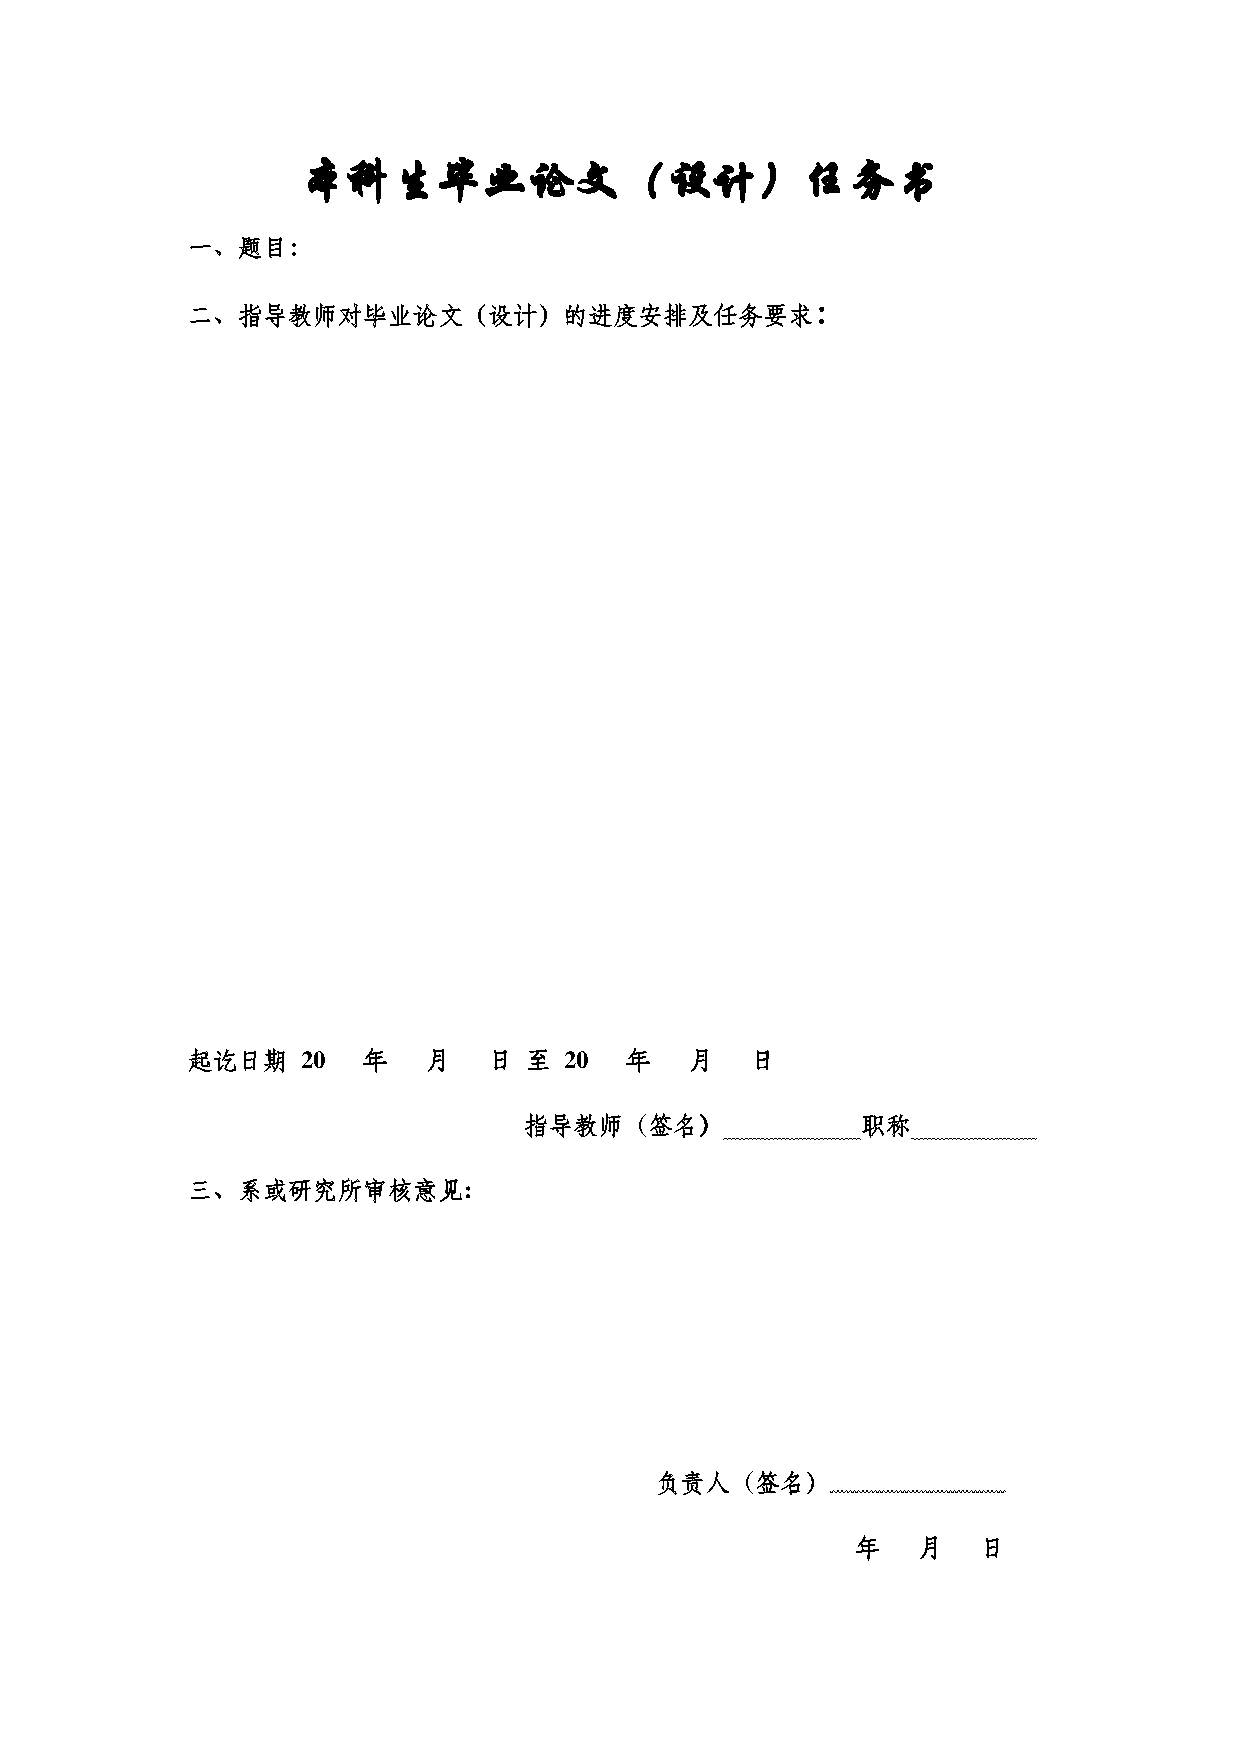
\includepdf[fitpaper=true,pages=-,pagecommand={\thispagestyle{empty}},addtotoc={
		1, alonepage, 1, 《浙江大学本科生毕业论文(设计)任务书》, task
	}]{../assets/official-1-task.pdf}
	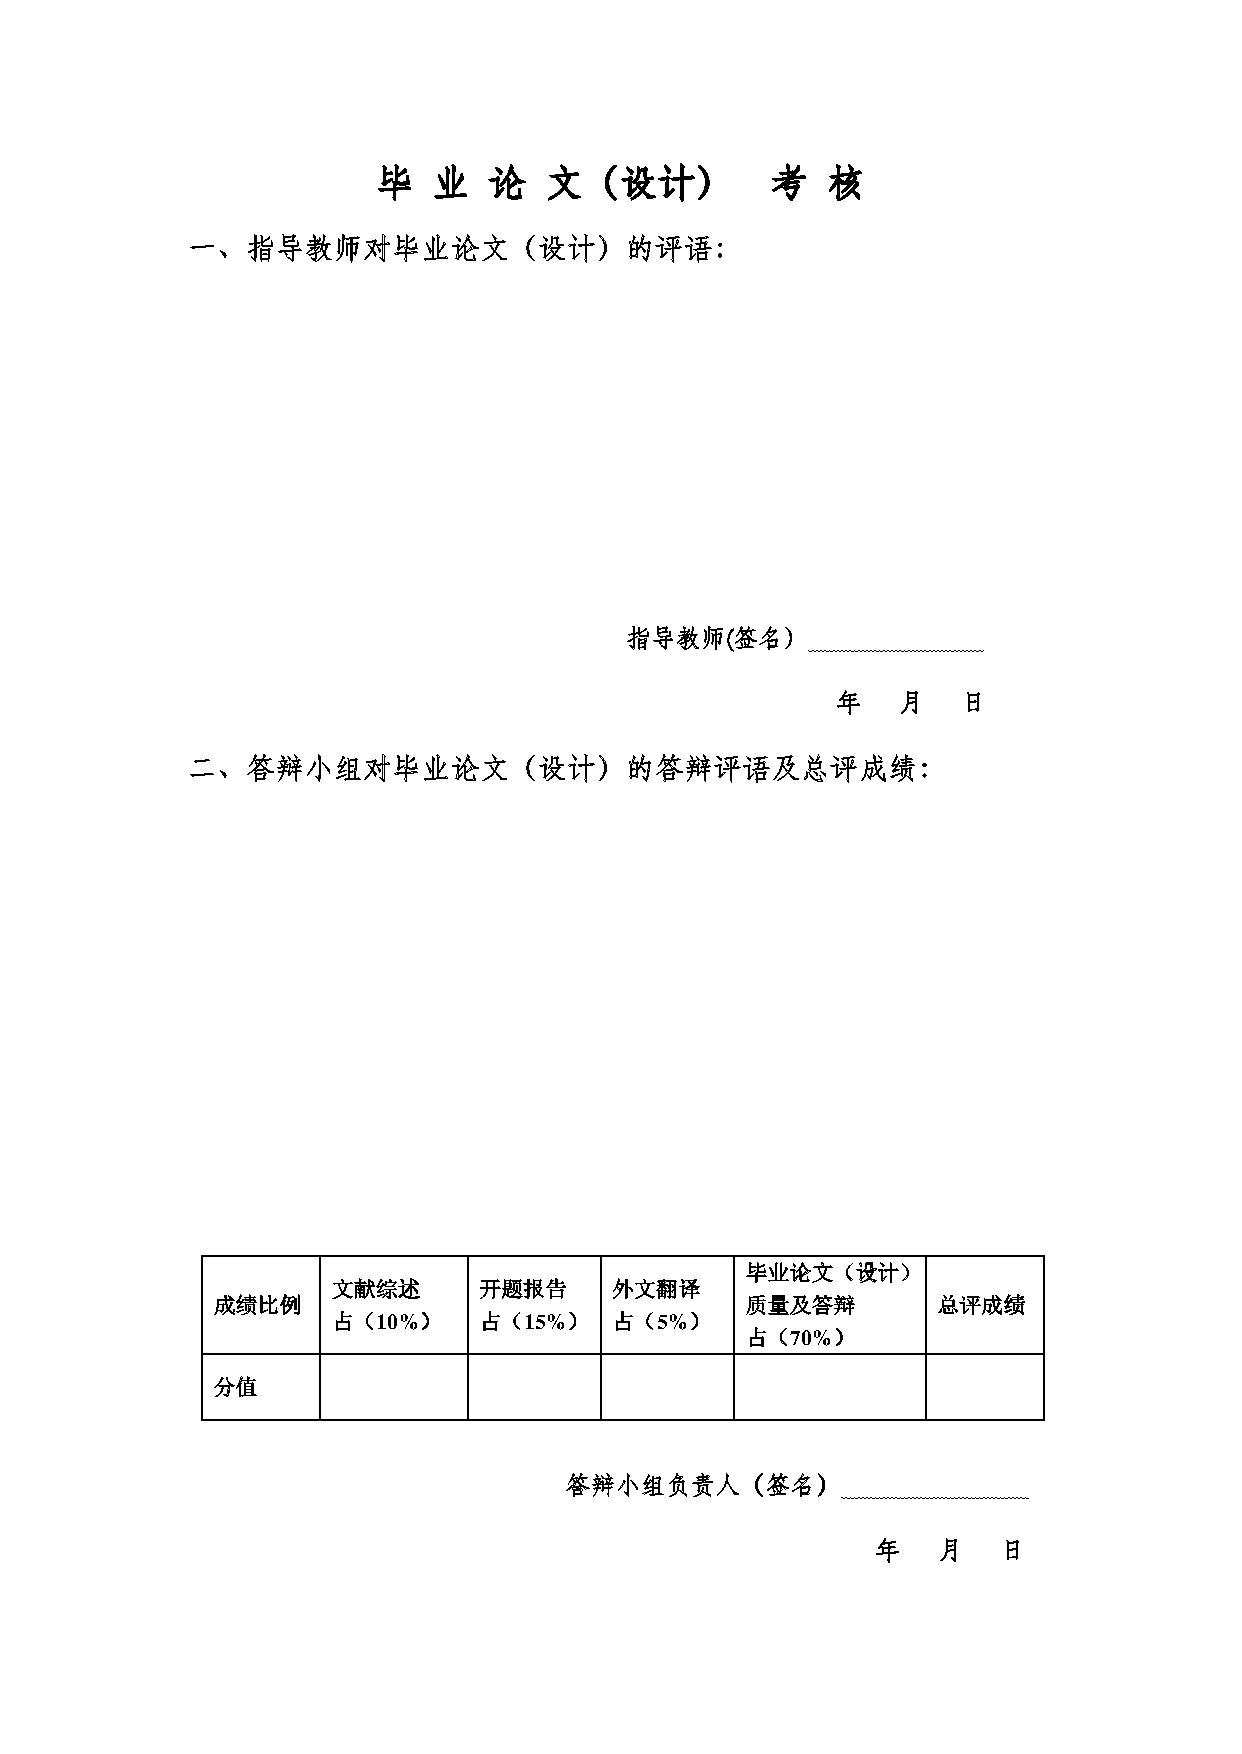
\includepdf[fitpaper=true,pages=-,pagecommand={\thispagestyle{empty}},addtotoc={
		1, alonepage, 1, 《浙江大学本科生毕业论文(设计)考核表》,assess
	}]{../assets/official-11-assess.pdf}
	\part{文献综述和开题报告}
	\renewcommand\thechapter{\zhnum{chapter}、} 
	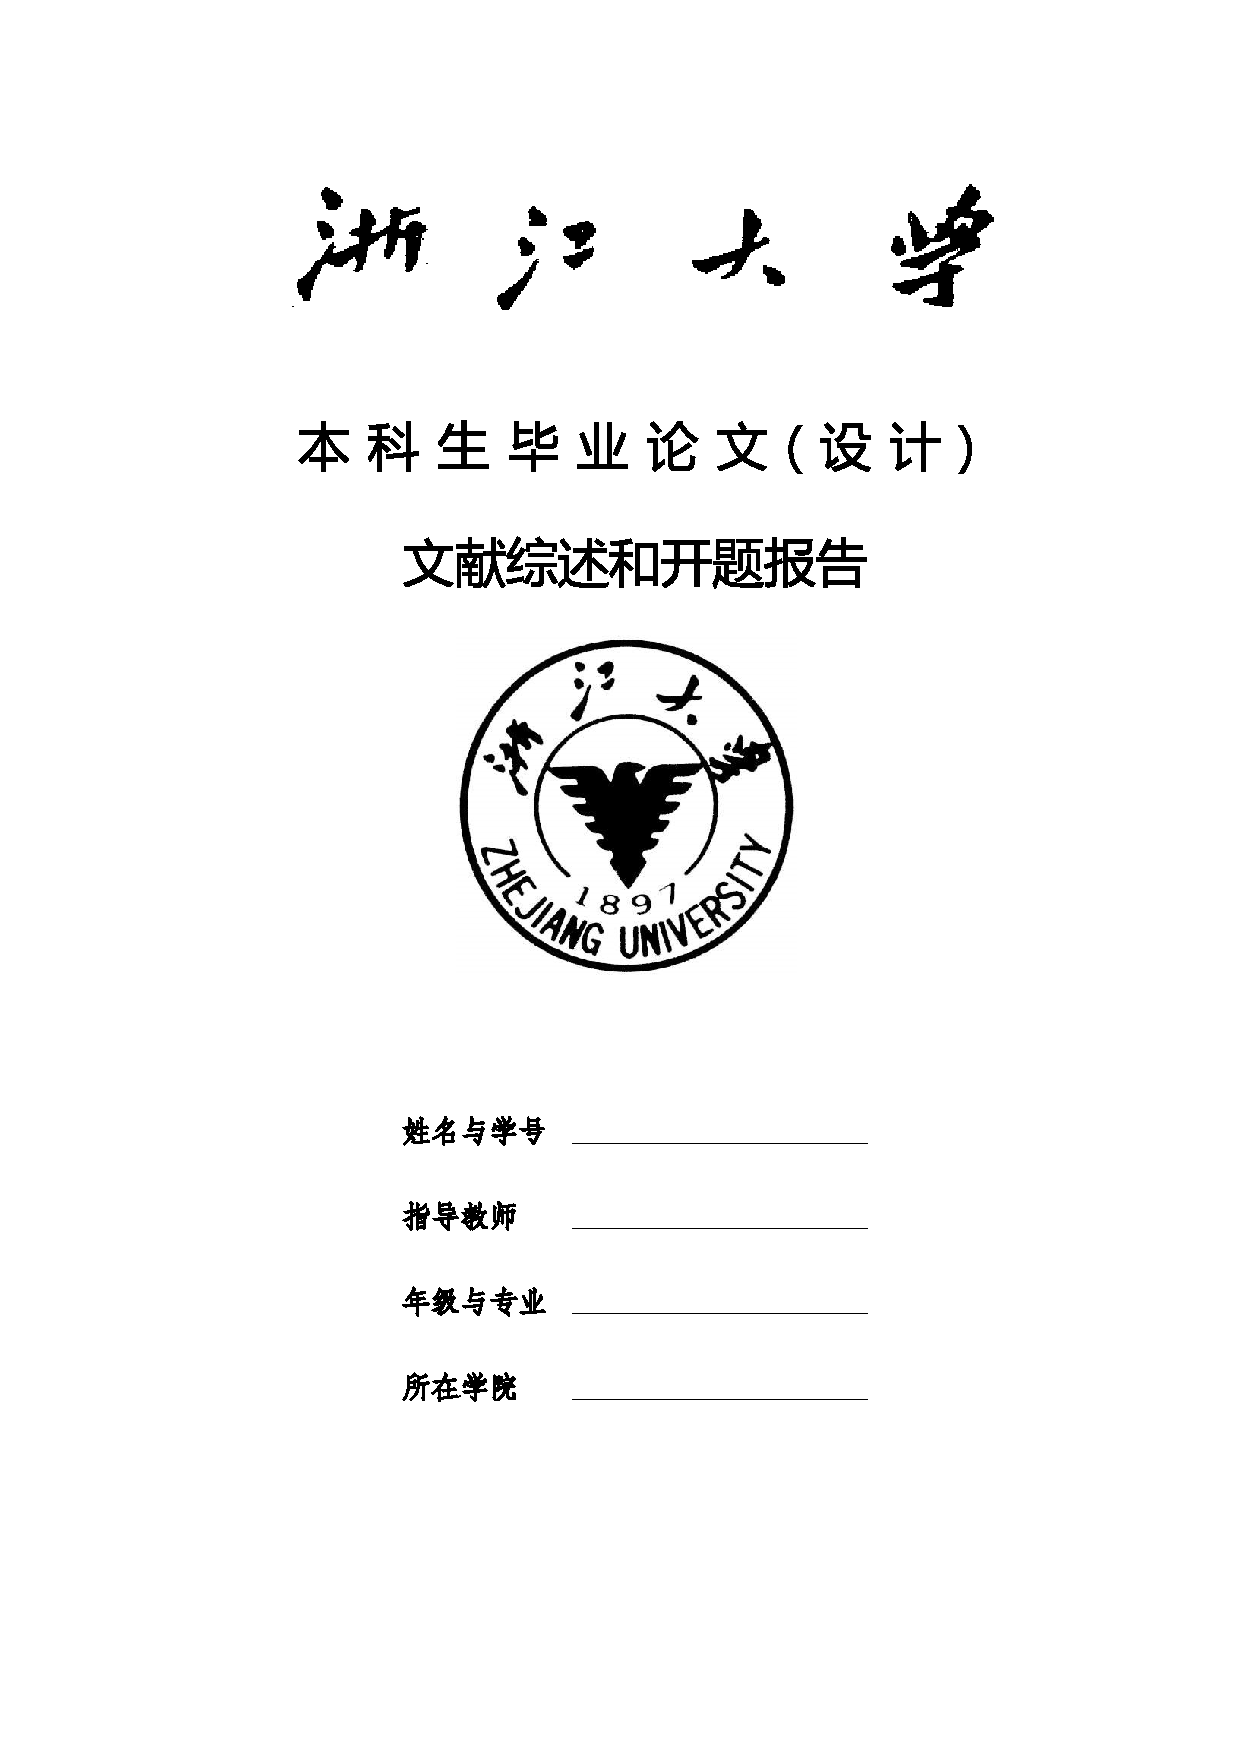
\includepdf[fitpaper= true,pages=-,pagecommand={\thispagestyle{empty}},addtotoc={
		1, alonepage, 1, 文献综述和开题报告封面, cover,
		1, alonepage, 1, 指导教师对文献综述和开题报告具体内容要求, cover,
		1, contabpage, 1, 目录,con,
		1, chapter, 1, 文献综述,s1,
		5, chapter, 1, 开题报告,s2,
		6, chapter, 1, 外文翻译,s3, 
		7, chapter, 1, 外文原文,s4,
		8, alonepage, 1, 《浙江大学本科生文献综述和开题报告考核表》,s5}]{../assets/proposal.pdf}
\end{document}